% TODO: tempted to term this "Module-aware dynamic fragmentation, analysis, and reassembly" as Dialysis or refracture
% CFP: https://www.usenix.org/conference/atc20/call-for-papers
\documentclass[letterpaper,twocolumn,10pt]{article}
\usepackage{usenix2019_v3}

\usepackage{soul}
\usepackage{xspace}
\usepackage{color}
\usepackage{booktabs}
\usepackage{graphicx}
\usepackage{alltt}
\usepackage{amssymb}
\usepackage{amsmath}
\usepackage{listings}

\lstdefinelanguage{js}{
  morekeywords={typeof, let, new, true, false, catch, function, return, null, catch, switch, var, if, in, while, do, else, case, break},
  keywordstyle=\color{purple}\ttfamily,
  keywordstyle=[3]\color{orange},
  keywords=[3]{SBX, PROC},
  ndkeywords={class, export, require, boolean, throw, implements, import, this},
  ndkeywordstyle=\color{cyan}\ttfamily, %bfseries
  identifierstyle=\color{black},
  sensitive=false,
  comment=[l]{//},
  commentstyle=\color{lightgray},
% morecomment=[s]{/\\*\\*, \\*/},
  stringstyle=\color{blue}\ttfamily,
  basicstyle=\footnotesize\ttfamily,  % the size of the fonts that are used for the code
  numberstyle=\tiny\color{gray},   % the style that is used for the line-numbers
  morestring=[b]',
  morestring=[b]",
% moredelim=[s][\color{gray}]{c:}{>},
% moredelim=[s][\color{orange}]{/*}{/}
}

\lstdefinelanguage{es}{
  morekeywords={string, number, bool, p, v, e, x},
  keywordstyle=\color{darkgray},
  keywordstyle=[3]\color{orange},
  keywords=[3]{SBX, PROC},
  ndkeywords={undefined, null, delete},
  ndkeywordstyle=\color{black}\ttfamily\bfseries,
  identifierstyle=\color{black},
  sensitive=false,
  comment=[l]{//},
  commentstyle=\color{lightgray},
% morecomment=[s]{/\\*\\*, \\*/},
  stringstyle=\color{darkgray}\ttfamily,
  morestring=[b]',
  morestring=[b]",
% numbersep=1pt,
% numberstyle=\footnotesize\bf\color{gray},   % the style that is used for the line-numbers
  abovecaptionskip=0em,
  aboveskip=0em,
  belowcaptionskip=0em,
  belowskip=0em,
  frame=none,                     % adds a frame around the code
% moredelim=[s][\color{gray}]{c:}{>},
% moredelim=[s][\color{orange}]{/*}{/}
}

\lstset{ %
  backgroundcolor=\color{white},   % choose the background color; you must add \usepackage{color} or \usepackage{xcolor}
  basicstyle=\small\ttfamily,  % the size of the fonts that are used for the code
  upquote=true,
  captionpos=b,                    % sets the caption-position to bottom
% frame=B,                    % adds a frame around the code
  numbers=left,                    % where to put the line-numbers; possible values are (none, left, right)
  numbersep=3pt,                   % how far the line-numbers are from the code
  numberstyle=\tiny\color{gray},   % the style that is used for the line-numbers
  rulecolor=\color{black},         % if not set, the frame-color may be changed on line-breaks within not-black text (e.g. comments (green here))
}


\usepackage{caption}
\captionsetup[figure]{font=footnotesize,name={Fig.},labelfont={bf, footnotesize}}
\captionsetup[table]{font=footnotesize,name={Tab.},labelfont={bf, footnotesize}, skip=2pt, aboveskip=2pt}
\captionsetup{font=footnotesize,labelfont={bf, footnotesize}, belowskip=2pt}

\usepackage{enumitem}
\setlist{noitemsep,leftmargin=10pt,topsep=2pt,parsep=2pt,partopsep=2pt}

\def\omit#1{}
\def\eg{{\em e.g.}, }
\def\ie{{\em i.e.}, }
\def\etc{{\em etc.}\xspace}
\def\vs{{\em vs.}\xspace}
% \newcommand{\heading}[1]{\vspace{4pt}\noindent\textbf{#1}\enspace}
% No vspace, coz Usenix class already has paragraph space
\newcommand{\heading}[1]{\vspace{2pt}\noindent\textbf{#1}\enspace}
\newcommand{\ttt}[1]{\texttt{#1}}
\newcommand{\ttiny}[1]{\texttt{\footnotesize #1}}
\newcommand{\tcn}[1]{}

\definecolor{cdb}{rgb}{0.37, 0.62, 0.63} % cadet blue

\newcommand{\cf}[1]{(\emph{Cf}.\S\ref{#1})}
\newcommand{\sx}[1]{(\S\ref{#1})}
\newcommand{\tb}[1]{(Tab.\ref{tab:#1})}
\newcommand{\rf}[1]{\ref{#1}}
\newcommand{\se}[1]{\S\ref{#1}}
\newcommand{\fg}[1]{Fig.~\ref{#1}}

\newcommand{\sys}{{\scshape Lya}\xspace}
\newcommand{\toy}{{\tt lya.js}\xspace}


\newcommand{\fra}{fragmentation\xspace} % fracture
\newcommand{\ana}{analysis\xspace}      % 
\newcommand{\ass}{reassembly\xspace}    % 
\newcommand{\Fra}{Fragmentation\xspace} % fracture
\newcommand{\Ana}{Analysis\xspace}      % 
\newcommand{\Ass}{Reassembly\xspace}    % 
\newcommand{\dia}{\fra, \ana, and \ass}

\newcommand{\R}{\ttt{R}\xspace}
\newcommand{\W}{\ttt{W}\xspace}
\newcommand{\X}{\ttt{X}\xspace}
\newcommand{\E}{\ttt{X}\xspace}
\newcommand{\rwx}{\ttt{RWX}\xspace}

% FIXME:
\newcommand{\pc}{PIC\xspace}
\newcommand{\pcs}{\pc{}s\xspace}

\newcommand{\goal}[1]{(\textbf{G#1})\xspace}

\newcommand{\nv}[1]{[{\color{cyan}#1 --- Nikos}]}
\newcommand{\review}[1]{{\color{red}#1}}
\newcommand{\TODO}[1]{\hl{\textbf{TODO:} #1}\xspace}
\newcommand{\todo}[1]{\hl{#1}\xspace}
\newcommand{\fixme}[1]{{\color{red}#1}}
\newcommand{\tc}{(\todo{cite})\xspace}
%-------------------------------------------------------------------------------
\begin{document}
%-------------------------------------------------------------------------------

%don't want date printed
\date{}

% make title bold and 14 pt font (Latex default is non-bold, 16 pt)
\title{\Large \bf Multi-library Program Dialysis with Lya}

%for single author (just remove % characters)
\author{
{\rm Anonymous Author(s)}\\
\normalsize{Submission \#225, 11 + 3 pages}\\
% \normalsize{Additional Anonymized Material: \href{https://git.io/JvfCf}{https://git.io/JvfCf}.}
% {\rm Grigoris Ntousakis}\\
% Technical University of Crete
% \and
% {\rm Nikos Vasilakis}\\
% Massachusetts Institute of Technology
}

\maketitle

\begin{abstract}

Applications today rely on hundreds of libraries, to the point where code written by their nominal developers is only a small fraction of their total line count.
Despite its benefits, this over-reliance creates many challenges, precisely due to the lack of knowledge and visibility into library internals---for example, in the presence of deeply-nested third-party code, security auditing and performance profiling, already challenging in monolithic applications, become extremely difficult.

To address these challenges, we present \emph{program dialysis}, a dynamic analysis technique specifically tailored to applications with many third-party libraries.
Combining name shadowing, context wrapping, and transformation of the underlying dependency graph, program dialysis automates dynamic fragmentation, analysis, and reassembly of programs at the level of individual libraries during program execution.
It bolts onto existing languages, enabling analysis expressions in the source language, with only a few lines of analysis-specific code.
Our dialysis prototype, \sys, targets the JavaScript ecosystem counting over 1M libraries for the web, server, and mobile.
We develop a series of case-studies that motivate \sys's design, and demonstrate how \sys allows the analysis of both individual libraries as well as multi-library programs with low developer effort and performance overhead:
  insightful analyses can be expressed in a few lines of code, add a minimal increase in the load latency of individual libraries, and scale to large programs with hundreds of libraries.

% Module dialysis can be bolted on existing language runtime environments in a language-agnostic fashion 
% % By leveraging the ubiquity of third-party modules in today's applications
% Such modules can be part of third-party packages or of the language's standard library;
%   the latter is important for resources that are part of the broader environment where the application is executing, such as the operating system and the network.

% Operating at this level of granularity has several benefits:
%   (i) it allows bolting library dialysis itself as a library onto existing runtime environments that do not feature dynamic analysis,
%   (ii) it supports analysis expressions directly in the same language, tools, and abstractions as the host application language---eschewing low-level instrumentation, and %developers can use their tools 
%   (iii) it features low performance overheads, to the point that has the potential to be used online.
% % FIXME: It depends on the analysis
% % Due to the in the host language and at a coarser granularity than full-fledged dynamic analysis, module dialysis 
% % Operating at the granularity of library has several benefits: (i) ease (ii) performance (iii) while still getting 
% %In a sense, modules are the right level of abstraction 
\end{abstract}

\section{Introduction}
\label{intro}

Dynamic analysis is a type of analysis performed by (and while) executing a program, with the goal of extracting information about the program and its execution.
Such information may include the ability to infer execution invariants, check security constraints, and extract performance characteristics~\cite{analysis:10}.
Contrary to other types of analysis, its key benefits make it the primary (or only) candidate in a variety of scenarios---namely, ones that require:
  (i) current runtime information, such as profiling data, in view of changing load patterns~\cite{staticdynamic},
  (ii) accurate visibility into the execution, devoid of abstraction or approximation~\cite{staticdynamic},
  (iii) Turing-complete policies, where monitors themselves are programs~\cite{contracts1, contracts2, contracts3},
  (iv) dynamic or runtime-reflection features, such as the ones present in Python and JavaScript~\cite{jsanalysis1, jsanalysis2}.

% Where dynamic analysis shines is
% Dynamic analysis occupies a clear spot in the space of analysis has clear strengths and weaknesses.
% Examples of information not analyzable statically include runtime code evaluation, runtime introspection and reflection, as well as multi-lingual support.
% Dynamic analysis is a particularly good fit for the analysis of dynamic languages.

Unfortunately, reaping these benefits comes with significant costs in terms of developer effort or runtime performance.
Manually instrumenting a program requires a good understanding of its internals. % instruction sets?
External tools such as instrumentation frameworks~\cite{pin, valgrind} and performance tracing tools~\cite{perf, dtrace} only add to the curve, as they feature their own language for specifying analyses. % usually different from the application's language.
Modifying the application's runtime environment such as the interpreter is cumbersome, error-prone, and requires development in a language that is different than that of the program.
Tools that virtualize execution~\cite{pin, valgrind, jalangi, roadrunner} have high performance costs---for example, Jalangi~\cite{jalangi} and RoadRunner~\cite{roadrunner} report No-Op analysis on the order of 26--32$\times$ and 52$\times$, respectively.
% Problem-specific solutions require significant investment outside the language's mental model---for example,  each ---as a case in point, Jalangi reports XX overhed (exact overheads always depend on the specific analysis).

Effort and performance costs are severely compounded by the use of third-party libraries, usually glued together without a full understanding of their internals.
This is a recent phenomenon enabled by zero-cost code sharing~\cite{libs}:
% Libraries are used pervasively today to lower development costs and improve software quality, 
% This over-reliance to third-party libraries is a recent phenomenon, 
  language-specific package repositories eliminate the cost of publishing and using a library.
As a result, applications frequently count hundreds of libraries~\cite{npmstudy:19}, with each one often only a few lines long~\cite{leftpad, npmstudy:19}. % how to say thousands of them depend on a 11-line lib?
Library-oriented analysis adds to the challenges of prior tools as
  (i) library boundaries disappear at runtime, and
  (ii) coarse-grained, high-level language semantics misalign with fine-grained, low-level instrumentation.

To address these challenges, we propose a novel approach to dynamic analysis, termed \emph{dialysis}\footnote{
  A method of deconstruction into elements often for the purposes of removing waste products or altering piecewise components.
  From ancient Greek {\scriptsize $\delta\iota\acute{\alpha}$} (di\'{a}, ``inter-, through'') and {\scriptsize $\lambda\acute{\tilde{\upsilon}}\epsilon\iota\nu$} (lúein, ``to loosen'').
} and implemented in \sys.
Program dialysis is a general technique, applicable to any programming language, that enables dynamic fragmentation, analysis, and reassembly of applications at the level of individual libraries. 
%                                                   !! sosto!!------.
%                                                                   \/
It operates during program execution, automating the wrapping and transformation of a program's dependency graph, and allows developers to extract meaningful insights with only a few lines of analysis-specific code.
By operating at the granularity of libraries, dialysis has several benefits over prior work: %full-fledged dynamic analysis:
  (i) it allows bolting analysis, itself as a library, onto unmodified runtime environments, % with no dynamic analysis,
  (ii) it supports analysis expressions using the same language, tools, and abstractions as the host program language,
  (iii) it features significantly low runtime performance overheads, enabling the potential for toggling its use in production environments.

% (i) at a somewhat coarser granularity, but still offering insights---and in a semantics-aware way tailored to the programming language.
% (ii) bolt on
% Our approach is applicable to any language that supports some notion of modularity, runtime introspection, and .
% It plugs into the module-loading capability of the runtime system to insert key hooks for inserting 
% After the parsing and interpretation phases of module loading complete, 
%  which are then parsed and interpreted and 
% Surprisingly, as we show in this paper, this architecture requires \emph{no} modifications to the language runtime---that is, it is backward-compatible with vanilla unmodified language runtime environments.
% 
% Its key strategy is to fracture applications at the boundaries of modules, instrument their interfaces (including direct accesses) using meta-programming capabilities, and recombine them 
% By combining visiiblity into both built-in and third-party modules, \sys can get gather important information for 
% at a much lower cost---both in terms of runtime performance and developer effort.
% 
% % to enable module-aware dynamic analysis are general
% To achieve this, module-aware dynamic analysis leverages several techniques.
% It plugs into the module manager;
% wraps interfaces
% (i) bolt on, meaning
% (ii) high-performance, and 
% (iii) low effort 
% 
% As shown later, these capabilities are generally available in all dynamic programming languages---\eg 

To demonstrate its effectiveness, we evaluate \sys on the JavaScript ecosystem (>1.2M libraries~\cite{modulecounts}). % and unusually high code-reuse~\cite{npmstudy:19}. %, and a pressing need for usable dynamic analysis~\cite{}.
We develop a diverse set of analyses that target practical information about a program:
  a read-write-execute security analysis,
  a profiling analysis showing bottlenecked modules,
% a synthesis-oriented analysis on input-output data,
  and an analysis extracting union-based type invariants.
These analyses drive the design requirements for \sys, and highlight dialysis as a middle ground between coarse- and fine-grained analysis.
We evaluate \sys at three different levels:
  (i) synthetic micro-benchmarks that test certain aspects and confirm the correctness of our analyses in a controlled environment;
  (ii) single-module meso-benchmarks that allow comparison with dynamic analysis frameworks; and
  (iii) end-to-end full-application macro-benchmarks that showcase \sys's behavior on realistic workloads. 
\S\ref{bg}--\ref{eval} present our key contributions:
\begin{itemize}
\item \S\ref{bg} characterizes the shared needs of three case-study multi-module analyses whose needs remain mostly unmet by general-purpose analysis frameworks.
\item \S\ref{design} presents the design of dialysis, bolt-on library-oriented dynamic analysis~\sx{design}, which meets the requirements of the three case-study analyses.
\item \S\ref{impl} discusses our implementation, \sys, as a pluggable library for the JavaScript ecosystem, as well as the implementation of the three analyses.
\item \S\ref{eval} evaluates \sys, showing that it expresses insightful analyses succinctly, adds minimal overheads over the baseline runtime, and scales to hundred-library programs.
\end{itemize}

Aside from the aforementioned sections (\S\ref{bg}--\ref{impl}), the paper discusses \sys's limitations and its application to other languages~\sx{diss};
  it compares with related prior work in the literature~\sx{rw};
  and draws appropriate conclusions~\sx{end}.


\section{Background, Examples, and Goals}
\label{bg}

A single application today often incorporates multiple libraries written and published by several different authors.
To make the difficulties of analyzing such library-overreliant software more concrete, we describe three example analyses~\sx{examples}.
These examples illustrate key requirements for the design of a framework for analyzing applications at the boundaries of modules~\sx{goals}.
Before describing these examples, however, we offer a brief refresher on the %abstractions and corresponding
  internals of a module system~\sx{bg1}.

% The emerging development process should (and to a certain extent, does) simplify the development and testing process;
%   unfortunately, good abstractions are sealed (\ie they do not leak between abstraction layers), which makes the inspection of a library difficult.

\subsection{Background on Module Systems}
\label{bg1}

\begin{figure}[t]
\raggedleft 
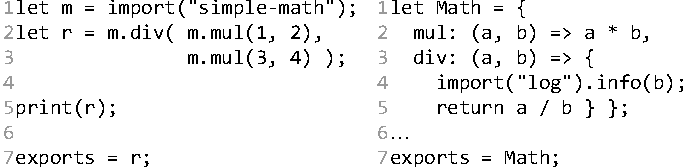
\includegraphics[width=0.45\textwidth]{./figs/lya_ex1.pdf}
\caption{
  \textbf{Example of a library import.}
  \textmd{
    The program on the left imports the \ttt{simple-math} library, shown right, which imports \ttt{log} and exports a \ttt{Math} object.
    Several names are provided by the programming language:
      \ttt{import} and \ttt{exports} resolve to library-local values; \ttt{print} resolves to a global value.
  }
  \vspace{-8mm}
}
\label{fig:ex1}
\end{figure}


A library, package, or module---we use these terms interchangeably---is a development-time construct encapsulating reusable functionality.
This functionality falls into two categories:
  it either (i) comes bundled with the language, possibly wrapping operating-system interfaces, such as the file-system, in a way that is system-agnostic and conforms to the language's conventions,
  or (ii) is provided by other developers sharing code others might find useful.
Fig.~\ref{fig:ex1} shows a \ttt{simple-math} library (right) imported by a program (left).

From a developer's perspective, \ttt{import}ing a library makes its functionality available to the calling code by means of binding its functionality to a name in the caller's scope.
% What this means is that some of the library's functionality is bound to a variable name that becomes available in the scope of the caller.
This is achieved by some form of \ttt{export}ing, where the library developer expresses which values should become available to the \ttt{import}ing code.
The definition of a value depends on the semantics of the language. % for now we can assume it's either a primitive value, a list of values, a function, or an object mapping string keys to values.
Internally, the library may \ttt{import} other libraries, cause side-effects to the file-system or the network, or even be implemented in multiple languages.
% , as shown on line \fixme{XX},
% closely coupled with the runtime
% and in some cases features its own mini-language, as is the case in Scheme and Standard ML.

From the programming language's perspective, the process of \ttt{import}ing a library is achieved in several steps. 
Compiled languages support separate compilation, where source files are compiled individually, followed by a runtime-linking phase that loads and links the resulting object files.
Interpreted languages involve a somewhat convoluted process that combines runtime loading, interpretation, and linking.
This process starts by locating the library in the file system, % or across the network,\footnote{
%   Examples of run-time environments featuring network loading include V8 and deno, for executing JavaScript and TypeScript respectively.
% }
by resolving code-relative module identifiers.
% The library is assigned a unique identifier.
The content of the library is then read and wrapped in a way that resolves library-local names, such as \ttt{\_\_name\_\_} in Python and \ttt{\_\_filename} in JavaScript, to meaningful values.
The wrapper is then interpreted and evaluated using the language's interpreter, which might result to side-effects---for example, a \ttt{process.exit()} in the library's top-level scope will exit the entire program.
Finally, the value bound to the \ttt{export}ed interface or returned from this interpretation (depending on the language) is made available to the scope of the  \ttt{import}ing code.

There is significant variation, but a few features are common across many implementations.
A library cache maintains a mapping from library identifiers, often absolute paths, to returned \ttt{export} values.
The cache serves a dual purpose:
  by avoiding locating already loaded libraries, it improves performance and ensures the consistency of any library-internal state.
Recursive imports are handled in a depth-first way, and when cyclical dependencies are possible, they are resolved by pointing to the cache.
An increasingly common feature is to allow different versions of the same library to co-exist in a program, in order to avoid a choice between mutually exclusive options---a paradoxical situation known as ``dependency hell''.
As a result, a single \ttt{import} $l$ does not necessarily resolve to the same (version of the) library $l$ every time.
The dual of this is also possible: two different library names may resolve to the same identifier (in which case the second will be redirected to the cache).
These features complicate library-level analysis, especially in interpreted programming languages.


% Several details:
%   same module at multiple levels, and the module cache
%   sometime it's the same, some times it;s not
%   module resolution algorithm

\subsection{Motivating Examples}
\label{examples}

Having reviewed the building blocks and underlying techniques that power modularity, we now turn to examples of dynamic analysis that today are difficult or require specialized solutions:
  (i) a read-write-execute security analysis,
  (ii) a performance-profiling analysis showing bottlenecked libraries, and
% (iii) a synthesis-oriented analysis on input-output data, and
  (iii) an analysis extracting runtime type invariants.
These examples illuminate key design requirements for dialysis in general and \sys in particular.
% \sys's implementation of module-level dynamic analysis.

\heading{Security Analysis}
The pervasive reliance on third-party libraries has led to an explosion of supply-chain attacks~\cite{long2015owasp, maass2016theory, snyk, lauinger2017thou}.
Both bugs and malicious code in libraries create attack vectors, exploitable long after libraries reach their end-users.
As library boundaries disappear at runtime, libraries end up executing with no meaningful isolation or privilege separation guarantees between each other and the trusted portions of a program.
Popular libraries, depended upon by tens of thousands of other libraries or applications, allow vulnerabilities deep in the dependency graph to affect a great number of applications~\cite{leftpad, npmstudy:19}.
Discovered vulnerabilities are becoming harder to eradicate, as updates are fetched automatically~\cite{npmFailure} and module unpublishing is becoming a multi-step process to avoid breaking applications~\cite{npmUnpublish}.
Worst of all, leaked publishing tokens allow attackers to update packages with code that will eventually reach end-users via package updates~\cite{eslint1}.

As a concrete example, consider the recent \ttt{event-stream} incident~\cite{es1, es2}, in which a maintainer of a highly popular library inserted code stealing Bitcoin wallet credentials from programs using that library.
Heavy-weight, offline dynamic analysis~\cite{jalangi} would not have helped, as \ttt{event-stream} activated only on production (rather than testing or development).
Coarse-grained analysis at program boundaries, say via containment or system-call interposition~\cite{systrace:03}, would have not helped either because host programs already used the network and disk.
Finally, static analysis would have been of little use, as \ttt{event-stream} encrypted its malicious payload.

Having the ability to toggle a library-level ``allow-deny'' security analysis on/off at runtime would have revealed the (unusual) resources touched by \ttt{event-stream}.
Analyzing the behavior \emph{within} the library itself is not critical:
  if any data exfiltration is happening, it will require calling out of the library and into the network---in \ttt{event-stream}'s case, using the \ttt{fs} library to modify a different library and then call \ttt{http} from the second library.
Both \ttt{fs} and \ttt{http} are part of the standard library, built into the runtime environment.
Examples of interfaces outside the \ttt{http} and \ttt{fs} libraries include the ability to use global variables, import other libraries, and access the cache of the loaded modules---all of which are unfortunately available to any third-party that is part of an application.
% The key issue underlying the \ttt{event-stream} attack is that any third-party fragment of an application has unrestricted access to the functionality available to the rest of application.

 %% To address such problems, several recent proposals suggest analyzing third-party modules dynamically to identify malicious behavior~\cite{}.
 %% % FIXME more about the policy, tracking arguments too
 %%  indicating the resources touched by that library 
 %% it seems critical to be able to toggle analysis on/off on production.
% \emph{
% This case highlights the need to \fixme{analyze} all the observable behavior \emph{around} a library, without necessarily caring about fine-grained library-internal analysis.
% }

\heading{Performance Diagnosis}
Diagnosing performance problems is a difficult task, exacerbated by the heavy use of third-party libraries.
Libraries are written by authors with different education, backgrounds, quality standards, and, most importantly, needs:
  it is not unusual for a weekend project solving a local need to end up as a critical dependency among several open-source projects~\cite{cheapcomplexity}.
Maintenance and rewriting can also cause performance regressions between two versions of a library;
% FIXME: Garbage collection
  worse even, the fact that a library changes one of its dependencies can cause severe performance pathologies to upstream projects---that is, while an interface remains the same due to an intermediate layer of abstraction, its performance can change dramatically~\cite{jest}.

As a concrete example, consider the \ttt{minimatch} library, a regular-expression-based file-matching utility susceptible to long delays due to regular expressions that involve backtracking~\cite{minimatch}.
Pathological inputs reaching \ttt{minimatch}, even if benign, can cause significant performance degradation~\cite{redos} deep in the dependency chain, affecting also other parts of the program competing for the same resources~\cite{evp}.
Developers use various techniques to understand such problems---\eg collecting and replaying traces against off-line versions of the system, or using statistical profiling to identify hot code-paths.
These techniques, however, require significant \emph{manual} effort:
  capturing traces, setting up test-beds, replaying traces, analyzing statistics, and debugging performance are all tedious and time-consuming tasks, compounded by the difficulties of mapping the results to the right third-party libraries.

Switching-on a library-level profiling analysis % that operates at library boundaries
  would quickly detect a slowdown and attribute it to the bottlenecked \ttt{minimatch}.
Wrapping library interfaces with profiling logic would collectively construct a model of the current workload.
Such profiling could operate at a high resolution in time and space---at every function call entering a library and on hundreds of libraries across an application---but does not need to track detailed operations such as direct variable accesses.
% An analysis could treat library invocation boundaries as message queues~\cite{scheme:98, duality:79} growing when a library gets overwhelmed.
% At some point, the waiting time of newly-arrived messages becomes longer than sending messages to a library replica.
Each library wrapper can collect profiling statistics at its own boundary, aggregating summaries into a global structure ordering libraries by resource consumption.


% \emph{
% This case highlights the need to \fixme{analyze} all the observable behavior \emph{around} a library, without necessarily caring about fine-grained library-internal analysis.
% }

\heading{Type Invariant Discovery}
Extracting type information in a program is helpful in a variety of different ways. %, as type safety is an important property helpful in variety of scenarios. 
%and types are lightweight annotations that can be quickly and efficiently checked.
For example, types can be used to (i) identify program invariants to be preserved during code modifications, (ii) generate (machine-checkable) program documentation, or (iii) guide program synthesis and regeneration~\cite{daikon}.
This is especially important in dynamic programming languages:
  in the absence of static type signatures, there is not much one can say about an object without executing it and inspecting its properties.

As a case in point, consider the \ttt{gRPC} library for serializing and de-serializing objects~\cite{grpc}.
To use it, developers have to provide a protocol-buffer specification describing the types of values that will be serialized.
Given a library---say, bignum or crypto---a developer has to first call it manually, take note of the result's type, and then fill in the protobuf spec. %, common in distributed systems
This process has to be repeated with every change, often due to library updates or changes in the consuming program's structure.

Library-level dynamic analysis can be used to discover such type assertions or invariants.
The analysis would consult the (static) definition of a type \emph{system}, capturing the type of values at the boundaries of libraries by observing their arguments during the execution of the program.
%% TODO: such as the simply-typed lambda calculus augmented with objects and union types.

% would need to be able 
% to capture structural subtitling---that is the piecewise 


% \heading{Learning, Synthesis, and Regeneration}

\subsection{Design Goals}
\label{goals}

We have briefly introduced three motivating analyses for extracting information about an application's dependencies.
While the challenges behind these analyses share several characteristics, today they remain largely unaddressed by dynamic analysis frameworks due to a combination of factors:
  these frameworks either require highly specialized solutions often outside the core language,
  do not leverage nor offer semantic information at the level of library boundaries, or
  lead to a high (often impractical) performance overheads due to the high granularity of their analyses.
To summarize, these applications would appear to be served well by a system that:
\begin{itemize}
  \item \textbf{(G1)} Operates at the level of libraries, leveraging both the semantics and performance potential that this level of granularity can potentially offer.
  \item \textbf{(G2)} Does not require learning a new tool or language, but rather allows developers to express their analyses in the same language as the program.
  \item \textbf{(G3)} Can be implemented as a library that bolts analyses onto an existing language runtime environment.
% \item \textbf{(G4)} It does not incur prohibitive overheads, such that it can be switched on and off selectively during runtime execution.
\end{itemize}

The next section describes program dialysis, a new analysis technique that satisfies these goals, in a language-agnostic manner~\sx{design};
  the section following that describes a concrete implementation for the server-side JavaScript ecosystem~\sx{impl}.

\section{The Design of Program Dialysis}
\label{design}

Dialysis starts by dynamically modifying the functionality of the module system that is responsible for importing and loading libraries:
  instead of simply locating and loading a library from the file-system, it yields control to \sys, which applies a series of transformations to libraries with the goal of interposing at their boundaries.
We start with an overview of dialysis~\sx{overview}, highlighting several key challenges, followed by a detailed description of each step~(\S\ref{one}--\ref{three}).

\subsection{Overview}
\label{overview}

% FIXME: add user data
Program dialysis operates by
  dismantling the program at the boundaries of libraries,
  applying transformations that insert analysis-specific machinery, and then carefully 
  reassembling individual components to maintain the original semantics:

\begin{itemize}
  
  \item \textbf{Fragmentation:}
Dialysis starts by recursively dismantling a program into its dependencies. % ---pieces of software implement a computation or functionality.
This is achieved by re-wiring the language's \ttt{import} function to go through \sys, resulting in \sys walking the program's recursive dependency structure at runtime.
During this phase, \sys has to determine the granularity of the analysis (\eg top-level libraries, a specific library \etc) in order to apply transformations at the correct level and map the provided analysis hooks to the corresponding libraries.

  \item \textbf{Transformation:}
It then sets up the provided analysis, by transforming each library interface, its surrounding environment, and possibly the values passing through the library boundary.
Programmatic transformations walk and wrap each one of these values based on their type.
% the library interface is usually a complex (but singular) object;
% the surrounding environment provides names to multiple ``implicitely'' imported libraries, functionality provided by the language.
This phase requires solving several challenges, including enumerating all points of entry into and exit out of a library, 
and swapping all original values externally-available to a library with ones that are wrapped with interposition mechanisms.

  \item \textbf{Reassembly}
Finally, dialysis reassembles individual modified libraries back into the program's original structure.
The most important challenge during this phase is the treatment of the library cache~\sx{bg1}.
The cache needs to be augmented to support multiple wrappers per library, each capturing a small fragment of the overall analysis.
% without breaking the program's semantics.
% ensure every fragment finds its place during dependency reassembly, 

\end{itemize}

% Program runtime transformations such as the ones applied in the second phase are used pervasively throughout \sys.

\begin{figure}[t]
\raggedleft 
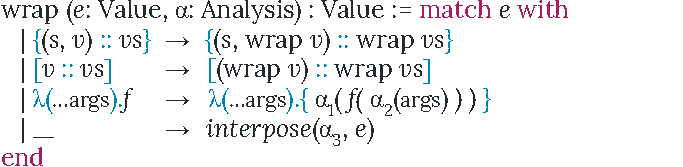
\includegraphics[width=0.45\textwidth]{./figs/lya_base.pdf}
\caption{
  \textbf{Base transformation.}
  \textmd{
  The algorithm (simplified) is presented in functional style to simplify variable binding; types (object, list, function, and primitive), used for pattern matching, are shown in light {\color{cdb} \emph{turquoise}}~\cf{two}. The functions $\alpha_1$, $\alpha_2$, and $\alpha_3$ stand for the locations of analysis hooks.
  }
  \vspace{-4mm}
}
\label{fig:base}
\end{figure}

% To transform a module, \sys augments several steps of the module loading process (Fig.~\ref{fig:pipeline}) using a base transformation that wraps an object with a security monitor~\sx{bt}.
% It starts by intercepting calls to the \ttt{require} function~\sx{import}, which locates the module's source code and \pc.
% It then constructs a custom context based on the \pc's implicit segment~\sx{context}.
% It then encloses the module in a closure to leverage local variable resolution in order to link the custom context with the module~\sx{enclosure}.
% After source interpretation, \sys transforms the resulting value by consulting the \pc's explicit segment~\sx{final}, updates the \sys-augmented module cache~\sx{cache}, and returns the value to the consumer.
% The following subsections detail these steps.

\subsection{Fragmentation}
\label{one}

When a dialysis-augmented program starts, it first loads the analysis file provided by the developer. 
The file may specify a subset of libraries whose boundaries are of interest or a subset of libraries that should \emph{not} be analyzed.
Among other things, \sys needs to determine the library boundaries of interest and the granularity of analysis.
To do this, it extracts a static approximation of the dependency graph by traversing library files.
Using this graph, it processes the analysis file to extract a mapping from library identifiers to analysis hooks.
It also checks for constructs not associated with libraries---for example, whether the analysis includes global variables, library-local constructs, standard libraries \etc
\sys then proceeds to dynamically replace the implementation of \ttt{import} and launch the program:
  rather than simply locating and loading a library, calls to \ttt{import} now yield to \sys.

For every invocation of \ttt{import} \sys checks the cache~\sx{three} to determine
  (i) if the library has already been loaded, and
  (ii) whether it has been loaded with the same analysis hooks.
If both are determined true, \sys retrieves the cached version of the library and returns the transformed \ttt{export}ed value.
If the library was loaded with a different analysis---say because there are different analyses applied to different parts of a dependency tree---\sys constructs the appropriate analysis and applies a transformation pass on a cached copy of the unmodified library~\sx{three}.
% \omit{---the common case---}
Otherwise, \sys first invokes the built-in library loader to locate the library.

The process of loading new libraries includes (i) a phase of reading the necessary source files and (ii) a phase of interpreting them, interspersed by applications of transformations~\sx{two}.
Reading files returns a string representation of the code; interpretation uses the language's runtime evaluation primitives to convert the code into an in-memory object.
% A series of transformations is applied before and after interpretation~\sx{two}.

%FIXME: Need to start with both problems
Some analyses may themselves make use of global variables, libraries, and other analyzable constructs.
As these will be part of the same execution context, \sys must note to avoid transforming and wrapping these constructs as part of the analysis.
% The analysis language is embedded in the source language, thus \sys makes use of the language's built-in evaluation primitives to interpret the \pc specification file.
Dialysis frameworks may also want to add analysis-specific keywords not provided by the language.
To achieve this, \sys wraps each analysis hook with a function whose body starts by defining the expected keywords.
The precise techniques for achieving this will be made clear in the next section~\sx{two}, after covering transformations;
  the key point to remember is that analyses are initially represented as source strings, similar to libraries.

\begin{figure}[t]
\centering 
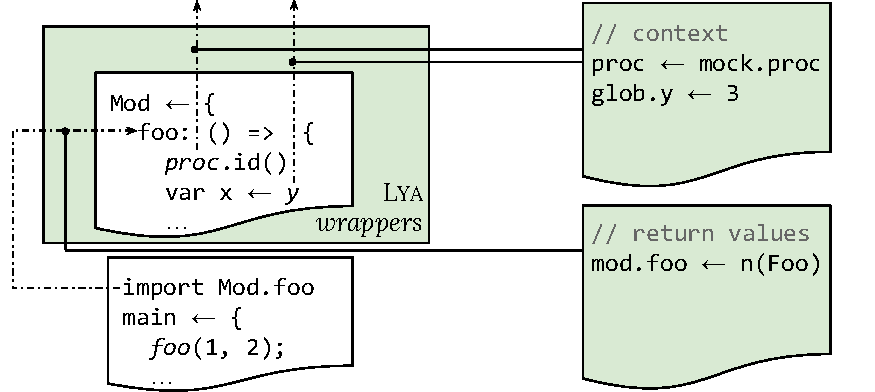
\includegraphics[width=0.45\textwidth]{./figs/lya_shadowing.pdf}
\caption{
  \textbf{Shadowing segments.}
  \textmd{
  Cross-module variable name resolution (left) augmented with \sys (green boxes), which interjects non-bypassable steps resolving to \sys-augmented values (right-top: implicit module imports; right-bottom: explicit import)~\cf{two}.
  }
  \vspace{-4mm}
}
\label{fig:shadowing}
\end{figure}


\subsection{Transformation}
\label{two}

%FIXME: Needs examples, especially the context
For each analyzed library, \sys needs to place hooks all around its boundary---not just its interface (Fig.~\ref{fig:shadowing}).
This is achieved in three logical steps:
(i) transforming library's context, a mapping from names to values that are available from outside library,
(ii) interpreting the library within this context, so that all names bind and resolve to \sys-augmented values, and
(iii) transforming the library's \ttt{export} value, \ie the library interface, once the interpretation is complete.
Before discussing \emph{where} each transformation is applied, however, we show \emph{how} they are applied.

\heading{Transformations}
% , such as an object returned from a module or an exception about to be sent across the network.
\sys's transformations boil down to a base transform \ttt{wrap} that traverses and augments values with runtime analysis monitors.
At a high level, \ttt{wrap} takes a value $v$ and analysis fragments $(\alpha_1, \alpha_2)$ and returns a new value $v'$ that has every one of its fields $f$ wrapped:
   every $f$ is replaced with a method $f'$ that calls fragment $\alpha_1$, calls $f$, calls fragments $\alpha_2$, and returns the result of the call to $f$.

More specifically, \ttt{wrap} can be applied to any value in the language, which can generally be a primitive, a function, or a compound value---say, a list of values or an object of key-value pairs.
% Listing~\ref{core-tx} presents a simplified core of the language.
Transformations walk compound values from their root, processing component values based on their types (Fig.~\ref{fig:base}):
% More specifically,
  (i) \emph{function} values are wrapped by closures that contain analysis-specific hooks; % on the function's arguments and return values;
  (ii) \emph{object} and \emph{list} values are recursively transformed, with their getter and setter methods replaced similar to function values; % and at times combining return results; and
  (iii) \emph{primitive} values are either transformed directly or copied unmodified and wrapped with an access interposition mechanism.
To avoid cycles during the walk, values are added to a map that is consulted at the beginning of each recursive call.
% Usually transformations do not mutate original values, but first copy them, apply transformations to the copies, and return copies to the caller.


% \sys's transformations boil down to a base form \ttt{BT} that augments \emph{objects} with runtime security monitors.
% At a high level, \ttt{BT} takes an object $O$ and a \pc $\sigma$ and returns a new object $O'$.
% Every field $f$ of $O$ is wrapped with a method $f'$ defined to enclose $f$.
% At runtime, $f'$ checks $\sigma$:
%  if the access is allowed, it forwards the call to $f$;
%  otherwise, it raises an exception.
% % Appendix: An example result is shown in the appendix.~\ref{fig:bt2}.
% 
% To achieve this transformation, \sys walks the object graph from the root and processes component values based on their types (Fig.~\ref{fig:base}).
% Rather than mutating original values, it copies them, applies transformations on the copies, and returns copies to the caller:
% 
% % Listing~\ref{core-tx} presents a simplified core of the language.
% 
% \begin{itemize}
% \item
%   \emph{function} values are wrapped by a closure that forwards arguments to the original function if allowed to do so.
% \item
%   \emph{object} values are recursively transformed, with their getter and setter methods replaced similar to function values.
% \item
%   \emph{primitive} values are copied unmodified and wrapped with an access interposition mechanism.
% \end{itemize}

Direct field accesses, such as assignments, require detection upon access.
To achieve this, \sys wraps fields with an interposition mechanism;
  this mechanism essentially treats direct field accesses as function calls (see \S\ref{impl} for implementation details and \S\ref{reqs} for equivalents in other environments).
% Examples of such mechanisms include \ttt{Proxy} objects (JavaScript), metatables (Lua), metaclasses (Python), and direct-accessor metaprogramming (Ruby).
Extending a transformed object with a value will start with the value's transformation.
% \sys's wrappers detect and record changes to any of the object's fields, transforming values as needed.
For example, if a field in a transformed object is assigned a new value, that value has to be transformed before it is attached to the object.

\sys allows toggling analyses on/off, changing analyses, or chaining multiple analyses during the execution of the program.
To achieve this, it maintains a handle to the root of both the unprocessed and the newly processed values, for further processing:
  the unprocessed value is used to create objects, at runtime, that run different analyses;
  the new value is used to revoke or chain analyses together.

\heading{Context Transformation}
To be able to track an analysis at the library boundary, \sys needs to provide each library with values that are augmented with interposition wrappers---and do this for all of the names to which a library has access.
This includes global and pseudo-global\footnote{
  For example, Node introduces objects that are not part of the EcmaScript specification into the global scope, such as \ttiny{process} and \ttiny{console};
  similarly, Lua's Luvit introduces its own globals such as \ttiny{p()} and \ttiny{exports}.
} names provided by the language and its runtime.

To achieve this, \sys first needs to prepare a transformed copy of the library's outer context.
Semantically, the context is a map from variable names to their values.
Thus, \sys creates an auxiliary hash table mapping names to transformed values.
Names correspond to any name that, by the language definition, is accessible by the library and resolves to a value outside that library, such as globals, built-ins, module-locals, \etc
Transformed values are created by applying \ttt{wrap} to values in the context, adding the provided analysis hooks.

%% FIXME: 
%% While user-defined global variables are stored in well-known locations,\footnote{
%%   For example, \ttt{globals} in JavaScript and \ttt{\_G} in Lua.
%% } traversing the global scope for built-in values is generally not possible.
%% To solve this problem, \sys collects such values by resolving well-known names hard-coded in a list;
%%   different lists exist for different environments and versions of the language.
%% Using this list, \sys creates a list of pointers to unmodified values. % upon startup.

Care must be taken with library-local variables. % that refer to library-specific information such as \ttt{\_\_name\_\_} in Python~\sx{bg1}.
These are accessible from anywhere within the scope of a library (similar to global variables), but resolve to a different value for each library.
Examples include the library's absolute filename as \ttt{\_\_name\_\_}, its \ttt{export}ed values, and whether the library is invoked as the application's \ttt{main} library~\sx{bg1}.
Attempting to access library-local variables directly from within \sys's scope will fail subtly, as they will end up resolving to library-local values of \sys \emph{itself}---and specifically, the module within \sys that is applying the transformation.
\sys solves this problem by leaving the value empty and deferring binding for later from within the scope of the library (see below).

\heading{Context Binding}
To link the library with the newly transformed version of its context, \sys wraps the library---still an uninterpreted string of source code---with a closure.
The closure's body starts with a prologue of the form:
\begin{verbatim}
  local print = ctx.print
  local error = ctx.error
  ...
\end{verbatim}
These statements shadow global variable names by redefining them as function-local ones.
The closure accepts an argument \ttt{ctx} that will hold the customized context (see above), assigning its entries to their respective variable names.
The prologue executes before everything else in the library.
% When the closure is applied to the customized context, the library's return value is recovered in a side-effectful manner (as in the unmodified library system) by reading the library's \ttt{exports} variable---that is, the closure does not end with an explicit \ttt{return}.
This technique leverages lexical scoping to inject a non-bypassable step in the variable name resolution process:
  instead of resolving to variables in the context, resolution will first ``hit'' library-local values augmented with analysis monitors.

Late-bound, \emph{library}-local variables, such as the absolute filename mentioned during context creation, are the result of applying \ttt{wrap} over variable names in the current scope;
  these names are now bound to the correct library-local values.

\heading{Library Interface Transformation}
Returning the library's value to its consumer amounts to interpreting the library, linking it with the custom context, and applying a final transformation to its return value.
% TODO: (for intro!) ..to attenuate the privilege exercised by the library's consumer
The goal of the final transformation is to track activity at the boundary.\footnote{
  For some analyses, \sys needs to additionally augment the values going through the library's interface---including continuation functions passed as arguments to the library's methods.}
This final transformation is applied for every new consumer of the library, returning a fresh analysis wrapper.
This is due to the need for distinguishing between different boundaries of the same library.

The treatment of this feature during reassembly is explained in the next section~\sx{three}.
  

\subsection{Reassembly}
\label{three}

To successfully reassemble the application, \sys needs to ensure that cross-references between libraries resolve correctly.
The central mechanism for this resolution is the library cache.

To support multiple wrappers for a single cached library, the cache is extended by two levels (for a total of three).
The reason for adding the two levels is that libraries are usually governed by a single context analysis but multiple interface analyses, one for each of their consumers.
A context transformation is applied at most a few times (usually only once), whereas a return-value transformation is applied on every \ttt{import}.
Thus, the first level is indexed by library identifiers (as before); the second by context analysis; and the third by analysis of the \ttt{export}ed interfaces.
% The first level is indexed by library identifiers as before, the second level is indexed by implicit segments, and the third level is indexed by explicit segments.
For each library, the second level contains a collection of entries corresponding to mostly-transformed libraries, and the third level contains fully transformed libraries.
Mostly-transformed libraries have gone through the entire transformation pipeline except for the last stage:
  they have been interpreted and have had their context transformed and linked, but their return value has not been processed to track analysis of its interface.

% A single augmented object (such as \ttt{Object}) may need to be shared among multiple files in a library, or even multiple libraries within a package directory.
A special entry is reserved for the original library value as a string~\sx{two}, so that subsequent transformations can skip loading the library from disk.
When a new analysis is applied to a library, \sys indexes the cache by library identifier and applies the analysis-specific \ttt{wrap} to the library's context.
It then adds that result to a slot in the next layer of the cache, indexed by the analysis identifier.
When a library is already loaded, \sys indexes by analysis to retrieve the (mostly) transformed library corresponding to this analysis.
It then applies a transformation to the library's return value, and inserts the (finalized) transformed library to the third layer of the cache.
% New libraries are inserted into the second-level cache right after evaluation of the interpreted function.


\section{Implementation of Dialysis for SSJ}
\label{impl}

\begin{figure*}[t]
\centering
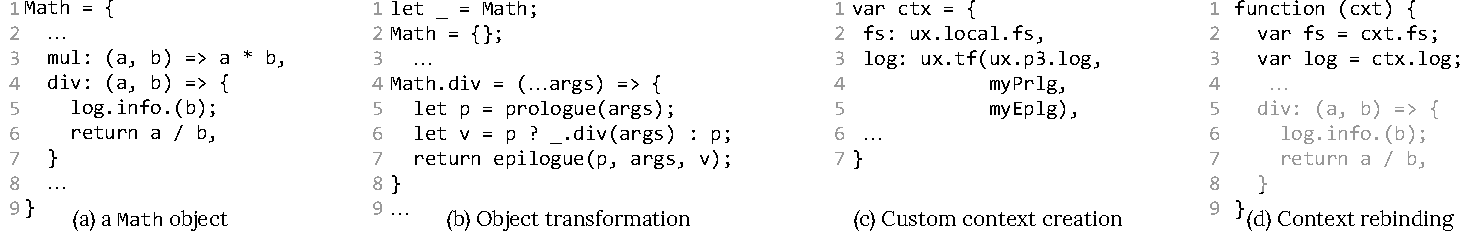
\includegraphics[width=0.99\textwidth]{./figs/lya_ex2.pdf}
\vspace{-2mm}
\caption{
  \textbf{Example transformations.}
   Applying runtime transformations (b) and context rebinding (c, d) on a simple \ttt{Math} object~\cf{impl}.
}
\label{fig:ex2}
\vspace{-4mm}
\end{figure*}

% Fixme switch from libraries to modules?

This section details our implementation of \sys for server-side JavaScript (SSJ) in about 1.5K lines of code on top Node.js v8.9.4~\sx{impl1}, and 
% We start with the internals of \sys's implementation, and then describe
including the three analyses developed atop \sys~\sx{impl2}.
Discussion of how other environments diverge from JavaScript is left for the next section~\sx{reqs}.

The aforementioned dialysis design can be implemented in either of two ways.
The first is to implement \sys as a modified version of the runtime, in which several stages of its library-loading facility have been augmented in-place. % with the techniques described earlier.
The second approach is to implement \sys as a third-party library (\eg the \ttt{lya} package) available by the language's package manager.
% 
With both approaches, \sys feels to users as a backward-compatible, drop-in replacement of Node's module system.
We went with the second approach, as looser coupling seems to have several benefits:
  it does not force \sys's users to have a Node copy only for running analyses;
  it removes \sys's developers from the critical path of updates between the Node developers and its users; 
  and it simplifies \sys's comparison with vanilla Node (both in terms of performance and correctness).
The primary drawback was missing a few opportunities for lowering runtime-performance and development-effort.

% It sketches the Node runtime~\sx{a}, the use of the module system~\sx{b}, and the internals of how module loading works~\sx{c}.

\subsection{System Implementation}
\label{impl1}


Node's module system is implemented entirely in JavaScript, exposing a library-local \ttt{require} function for importing modules.
Loading a fresh module % with \ttt{require("foo")}
  corresponds to the following five stages, all of which are augmented by \sys:
(R) Resolution: identify the file to which the module specified corresponds, locate it in the file-system, and assign its absolute path as a module identifier.
(L) Loading: depending on the file type, identify the corresponding loader---\eg V8 compiler for \ttt{js}, \ttt{JSON.parse} for \ttt{json} \etc
% Identifiers are absolute paths.
(W) Wrapping: wrap the module so that local names do not escape the module's scope and Node's module-local names get resolved.
(E) Evaluation: evaluate the wrapped module in the current context, so that global names and top-level objects get resolved correctly.
(C) Caching: add the module to a handful of module-related caches, for purposes of consistency and performance.

% The resolution algorithm is somewhat convoluted, because it depends on several different facts (including the type of the file requested, whether it is a globally installed, whether it is a directory \etc).
% It does not require any \sys support beyond copying the directory that contains the source code of the all the modules onto the remote host.
% \sys interposes on all of these steps to facilitate transformations.
\sys augments all of these steps.
Interposing on resolution (R) makes the module identifier available to \sys without affecting the (incredibly convoluted!) module resolution algorithm.
If the module's type corresponds to a module that can be analyzed by \sys, \sys fetches the corresponding analysis during loading (L).
Wrapping (W) and evaluation (E) are where \sys transforms the module boundary.
\sys replaces Node's wrapper function to pass an additional argument, the modified context \ttt{CTX}.
\sys comes with a hard-coded list of names corresponding to the specific versions of EcmaScript and Node.
Identifying names coming from EcmaScript was relatively easy, as the standard makes them explicit.
Node's global names are described at various parts of the documentation, but library-local names required close inspection of Node's internals; fortunately, they were only five names.

% Before a module's code is evaluated, the Node.js module loader wraps the module so that
%   (i) it keeps top-level variables (declared with \ttt{var}, \ttt{const} or \ttt{let}) scoped to the module rather than the global object; and
%   (ii) it provides some global-looking variables that are actually specific to the module, such as the \ttt{module} and \ttt{exports} objects that the implementor can use to export values from the module and convenience variables---such as \ttt{\_\_filename} and \ttt{\_\_dirname}  containing the module's absolute filename and directory path, respectively.
% True globals remaining are
%   (i) the global objects as defined by the EcmaScript standard (\eg \ttt{Object}, \ttt{Function}, \ttt{Math}); and
%   (ii) Node.js-specific globals (\eg \ttt{console}, \ttt{process}, \ttt{timer}).
% These globals require further interposition.


% TODO: Talk about recipe file, that could be kept along with the module identifier

% \begin{lstlisting}
% let lib = `
%  function (exports, require, module,
%            __filename, __dirname, CTX) {
%    let Math = CTX.Math
%    let console = CTX.console
%    //...[more definitions]
%    ${moduleSource}
%  });`;
% \end{lstlisting}

We found it useful to add an option for white- and black-listing libraries.
The configuration object accepts \ttt{only} and \ttt{not} expressions that indicate whether a module identifier will be part of the analysis.
These expressions contain sets of regular expressions, pattern-matching against module identifiers, which in Node are represented as absolute file-system paths.
Originally intended as an aid to \sys's development and debugging, this option proved useful enough for writing the three analyses that we decided to expose it to \sys's users.
Examples of its use include blacklisting built-in libraries or white-listing only the library imported most recently.
% This is useful, for example, when...

% get second argument, no need to pass arguments around, tricky to 
% carefull hardcoding of paths, because \sys's code itself is split into modules

%% TODO: implementation

Fig.~\ref{fig:ex2} exemplifies \sys's transformation techniques in the context of JavaScript.
\sys traverses a \ttt{Math} object, replaces functions such as \ttt{div} with wrappers, creates a modified version of the surrounding context, and binds it to the library.


\subsection{Individual Analyses}
\label{impl2}

Individual analysis are implemented using a set of templates that provide initial constructs.
%% Individual transformations described earlier~\sx{overview} are in \sys  abstracted by a set of parametrizable skeletons.
%% These skeletons provide hooks for end-developers writing analyses.
%% Specifically, they map types of values (\eg \ttt{Number}s, \ttt{Function}s) to generic hooks for each type. 
%% These hooks are then extended or rewritten by developers to
\sys offers a small utility library to reduce boilerplate code for pattern-matching on types.
Individual analyses are about 60 lines of code, but a significant part of this code is common across them.

As the three analyses are quite complex to include in the paper, we present here a trivial analysis---one that counts all accesses to global variables from a module \ttt{serial}:

\begin{lstlisting}
let fs = require("fs");
let count = {};
forevery.global.in(/serial/).do({
  pre: (name, path, _) => {
    let o = resolve(name, path);
    count[o] = count[o]?  count[o] + 1 : 1;
  } });
process.on("exit", () => {
  fs.writeFileSync("acl.json",
                   "utf-8",
                   JSON.stringify(count)); });
\end{lstlisting}

\noindent
\sys-provided \ttt{forevery} generates sets of names succinctly.
The \ttt{in} field is a method that takes a regular expression matching module identifiers.
If not empty, \ttt{pre} and \ttt{post} hooks are called before and after each access of the elements specified in the set.
Finally, \ttt{resolve} is a method for traversing an object given a path within that object.
Upon program exit, the results are written to disk, all using the expected Node APIs.

\heading{Security Analysis}
To address the security concerns of third-party libraries, we developed a concrete \ttt{RWX} policy that analyzes accesses for every library-to-library combination.
The analysis treats built-in libraries and global variables as modules,
% and generates a list of permissions for each of their fields.
and develops a permission model where individual fields are governed by permission sets containing combinations of read, write, and execute permissions:
 (i) a read permission (\R) indicates that a consumer read a value, including assigning it to a variable and passing it around to other modules;
 (ii) a write permission (\W) indicates that a consumer modified or deleted a value; and
 (iii)  an execute permission (\X) indicates that a consumer executed a value---\eg a function or a method---or invoked a constructor (usually prefixed by \ttt{new}).

The resulting permission sets are organized as collections of maps, one per library, indexed by object-paths---\eg \ttt{require("Math").add: RX}.
% that correspond to values of other modules or global-like language names.

\heading{Performance Diagnosis}
We developed a profiling analysis that operates at two levels:
 (i) module-boundary wrappers that collect profiling statistics for calls between modules by wrapping module interfaces; and
 (ii) an aggregator function that collects statistics from all boundary wrappers and generates a model of library load under the current workload.

Boundary wrappers operate at a higher-frequency intervals than the aggregator, which operates on summaries.
Their analysis focuses on function calls, skipping all other direct field accesses.
Functions are wrapped with prologue and epilogue wrappers that record statistics from the Node.js runtime---for now, a frequency counter and a timer between prologue-to-epilogue invocations.
% Many statistics are available by the Node.js runtime, including memory and garbage-collection statistics, 
Boundary wrappers summarize these statistics by periodically sending a windowed, weighted average of call latencies to the aggregator function.

% Wrappers record statistics about the their encapsulated functions as well as queue characteristics of outstanding calls.
% The wrapper epilogue has access to several raw metrics related to profiling (Tab.~\ref{tab:metrics}).
% These metrics are viewed as a windowed average that priori 

Interestingly, profiling functions at the boundary cannot ``see through'' libraries to correctly attribute load among a library and its dependencies.
For example, a boundary wrapper \ttt{A} of a dependency tree \ttt{A}$\rightarrow$\ttt{B}$\rightarrow$\ttt{C} does not know how much of the latency comes from \ttt{B}.
Fortunately, the aggregator understands the dependency structure and can approximate how much of the latency comes from each module.
% Such a approximation is more complicated than a simple subtraction, as a module may invoke interfaces from multiple modules at the same time.
% Having an analysis fragment per library consumer, however, alleviates much of the problem.

% FIXME: Snapshot results
% [serial , whatever, pizza, ...]

\heading{Type Invariant Discovery}
To infer type invariants for serialization specifications, we based our analysis on a simple type system modeled after the simply-typed lambda calculus augmented with:
  (i) unions (sum types), such as \ttt{string | number}, 
  (ii) JavaScript-specific types such as \ttt{null}, \ttt{NaN}, or \ttt{undefined}, and
  (iii) a \ttt{native} type for values that cannot be serialized, such as \ttt{console.log}.
Support for union types is useful for when our analysis witnesses variables holding values of different types---although, in practice,  programs tend to make calls of the same type across their entire lifetime~\cite{daikon}.

Our implementation also uses a base set of JavaScript types and rules to deconstruct complex types into their elementary building blocks.
% Knowing how to deconstruct a type to its structural primitives allows walking values---
For example, it unpacks a type \ttt{user} into two \ttt{string}s (first and last name) and a \ttt{number} (age).
% To achieve this, the analysis makes use of introspection to identify 

% leftpad: (string | number) -> number -> (string | null) -> string 

% \subsection{Limitations}
% 
% % FIXME: Talk about the inability to 
% A limitation of our implementation is that it cannot analyze the library importing \sys---usually, the top-level program entry-point equivalent to \ttt{main}.
% This is because \sys cannot transform the context of that file
% As a result, \sys as-is cannot be applied to, say, to analyze single-file programs---a common pattern in scripting languages often used for quick-and-dirty tasks.
% The simplest workaround here is to create an auxiliary file that imports \sys, and then import the single-file script (which, in most scripting languages would invoke it).

\section{Evaluation}
\label{eval}

\sys's  development achieves goals \textbf{G1--3}~\sx{goals}, demonstrating that it is indeed feasible to build a framework that 
  operates as a library around an existing runtime,
  does not require learning a new language, and 
  gets meaningful information while operating only at library boundaries.
% Despite the fact that it operates at coarser granularity, as shown earlier~\sx{impl} \sys can express analyses that generate results useful in several practical scenarios.
In this section, we report on \sys's performance characteristics:
% At a high level, we are interested in three questions:
  (i) the overheads of its underlying building blocks;
  (ii) dialysis on real libraries, and how they compare to a production-grade dynamic analysis; and
  (iii) \sys's behavior on realistic  multi-library applications.
% For the first question, we use  synthetic micro-benchmarks that built to stress key elements of the system and confirm it works correctly~\sx{micro}.
% For the second question, we use real libraries and compare them with an analysis written in Jalangi~\sx{meso}.
% For the third question, we use a combination of real applications~\sx{macro}.

Several takeaways are worth highlighting.
Analyses expressed in \sys are about 4$\times$ smaller than equivalent analyses written for a heavy-weight instrumentation framework.
\sys's library-level analysis adds a small overhead, less than $2\times$ for the vast majority of libraries and often less than $5ms$.
Finally, \sys scales to large applications with hundreds of libraries while interposing on several thousands of objects.

Experiments were conducted on a moderate server with 4GB of memory and 2 Intel Core2 Duo E8600 CPUs clocked at 3.33GHz.
In terms of software, we used Docker version 18.09.7 running a minimal Ubuntu 14.04.6, Jalangi v2, Node.js v8.9.4 (bundled with V8 v6.1.534.50, LibUV v1.15.0, and npm v6.4.1), all atop a Debian Linux with kernel v4.4.0-134.
All times reported are in \textbf{ms}, averaged over 1K runs;
  \textbf{SA}, \textbf{PD}, and \textbf{TID} respectively stand for security analysis, performance diagnosis, and type invariant discovery.
  

\subsection{Micro-benchmarks}
\label{micro}

\sys's micro-benchmarks were designed to test key properties of each analysis and confirm it outputs the expected results.
For example, to better understand PD and confirm it works correctly, we crafted a micro-benchmark with four dependencies of known static bottlenecks.
% Each dependency can perform one of three operations, depending on its current state:
%   (i) invoke a call to a module it imports,
%   (ii) busy-wait for a specific amount of time, or
%   (iii) respond to calls by returning a value.
A second goal was to understand \sys's internal overheads in a controlled environment.
% Both of these goals would have been difficult to achieve outside a controlled environment. % , as we do not fully understand applications we haven't written ourselves.

\begin{table}[t]
\center
\footnotesize
\setlength\tabcolsep{3pt}
\caption{
  \footnotesize{
    \textbf{Synthetic Micro-benchmarks}.
		Applying the three analyses on a series of synthetic micro-benchmarks, created to stress different features.
    All timings are in $ms$~\cf{micro}.
  }
}
\begin{tabular*}{\columnwidth}{l @{\extracolsep{\fill}} lll l}
\toprule
	               &   Base    &  SA     & PD      &  TID    \\
\midrule
globals vars     &   0.90    &  4.70   &  4.54   &  4.30   \\
built-in fields  &   1.44    &  6.46   &  6.24   &  5.96   \\
counter          &   3.37    &  6.26   &  6.32   &  5.72   \\
all names        &   7.79    &  13.54  &  13.31  &  12.8   \\
custom delays    &   24661   &  24848  &  24754  &  24760  \\
direct-access    &   4.06    &  7.24   &  7.16   &  6.79   \\
timple-types     &   4.11    &  7.25   &  7.23   &  6.86   \\
cycles           &   4.32    &  8.32   &  8.19   &  7.73   \\
\bottomrule
\end{tabular*}
\label{tab:synthetic}
\vspace{-5mm}
\end{table}

Table~\ref{tab:synthetic} depicts the results of the three analyses applied to a subset of our benchmarks.
The first column indicates the focus of the benchmark; not all analysis--benchmark combinations are useful.
% Currently, these benchmarks return the results we expect, but they did help with the identification of \sys's bugs.
For example, the ``custom-delay'' benchmark, described earlier, features static bottlenecks across its dependency tree but does not involve interesting access patterns.
The use of \sys adds an overhead that is under 2$\times$, except for the first two cases that feature \emph{only} accesses.
Close inspection confirms that overheads are proportional to the number of wrapped objects and the frequency of accesses:
  most of these benchmarks feature artificially tight loops with high-frequency accesses.
Transformation overheads themselves (not shown in Tab.~\ref{tab:synthetic}) remain under $1ms$.
% is not affected significantly % by transformations altering a library's context 

To understand the costs of proxy interposition, we measure the time to access deeply-nested properties of two versions of an object:
  unmodified and proxy-wrapped.
Paths to the properties (\eg \ttt{a.b.c.$\ldots$}) are random but generated prior to running the experiment.
We construct 500MB-sized objects, each with a fanout of 8 fields nested for 12 levels.
The proxy-wrapped version introduces interposition at every level.
Traversing one million 12-edge paths (\ie root to leaves) averages 167.2ms and 595.7ms for the unmodified and proxy-wrapped versions, respectively.
% 
We emphasize that this is an artificially constructed benchmark stressing worst-case overheads nowhere near an normal execution:
  for comparison, the transformation of these objects itself took nearly 16 seconds ($10^3\times$ more than what we saw with real modules).
The takeaway is that \sys-inherent overheads due to interposition are unlikely to be the bottleneck of an analysis;
  what is likely to be is the analysis itself---\eg updating a global aggregator or invoking system-calls to extract timing.

\begin{table}[t]
\center
\footnotesize
\setlength\tabcolsep{3pt}
\caption{
  \footnotesize{
    \textbf{\sys-augmented single-library programs}.
    The table shows the overheads of applying the three analyses to the test suites of eight libraries. % (with Minimist involving five test cases).
  }
}
\begin{tabular*}{\columnwidth}{l @{\extracolsep{\fill}} lll l}
\toprule
                               & Base   &  SA   & PD     &   TID   \\
\midrule
Classnames~\cite{classnames}   &  2.72  & 6.62  &  6.61  &  6.10   \\
Debug~\cite{debug}             & 31.39  & 33.54 &  33.94 &  33.96  \\
Minimist~\cite{minimist}       &        &       &        &         \\
~~~-t1                         & 31.46  & 60.13 &  60.00 &  56.62  \\
~~~-t2                         & 29.35  & 56.30 &  53.98 &  53.17  \\
~~~-t3                         & 30.34  & 59.13 &  55.76 &  55.34  \\
~~~-t4                         & 30.04  & 56.40 &  53.68 &  53.27  \\
~~~-t5                         & 30.24  & 58.17 &  55.07 &  54.76  \\
Moment~\cite{moment}           & 31.73  & 48.04 &  49.23 &  44.95  \\
yargs~\cite{yargs}             & 14.59  & 15.68 &  15.49 &  15.54  \\
chalk~\cite{chalk}             & 17.37  & 24.42 &  26.01 &  26.32  \\
colorette~\cite{colorette}     & 08.10  & 13.85 &  13.41 &  13.16  \\
mkdirp~\cite{mkdirp}           & 116.37 & 1959.52 & 1392.64 & 1252 \\
\bottomrule
\end{tabular*}
\label{tab:meso}
\vspace{-5mm}
\end{table}



\subsection{Single-Library Benchmarks}
\label{meso}

\begin{figure*}[t]
  \centering
   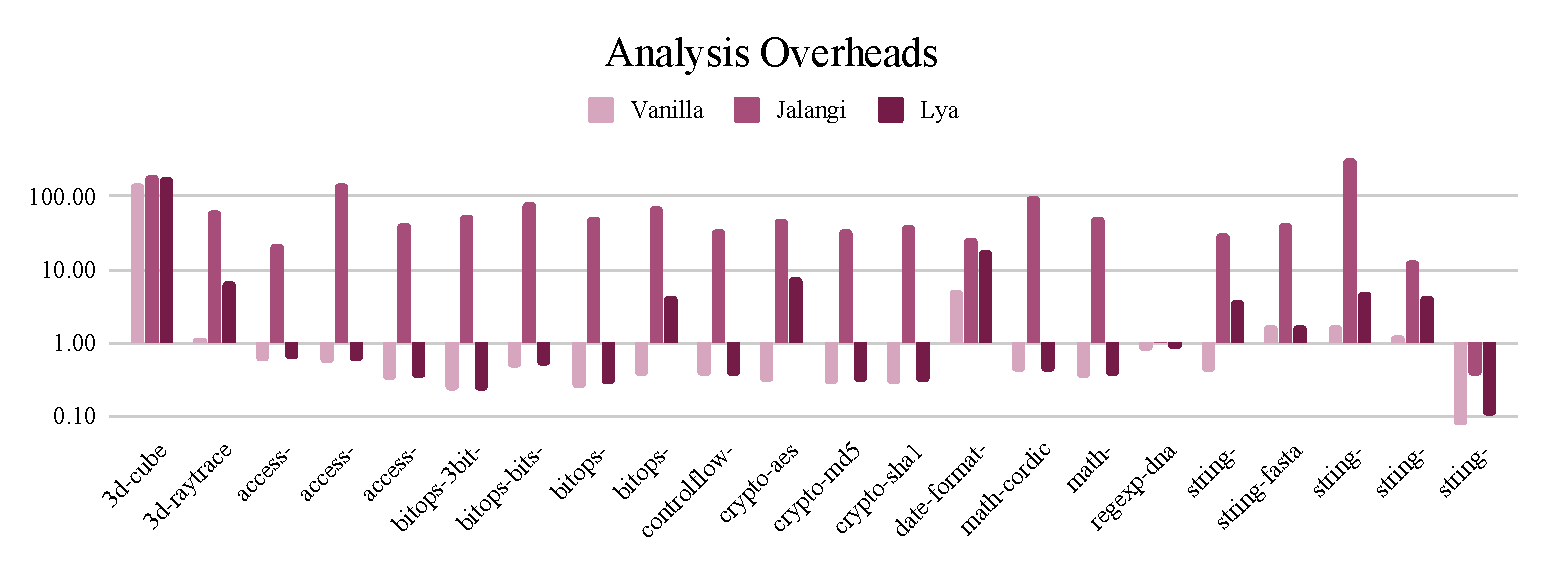
\includegraphics[width=0.95\textwidth]{./figs/meso.pdf}
  \caption{
    \textbf{Analysis overheads.}
    The plot compares single-library programs taken from Jalangi2 between three setups:
		(i) Vanilla JavaScript, (ii) global-use analysis with Jalangi2, (iii) global-use analysis with \sys.
    Global-use analysis is a simple analysis that tracks accesses of global variables in the program~\cf{meso}.
  }
  \label{fig:meso}
  \vspace{-3mm}
\end{figure*}


To understand \sys's performance characteristics at the level of individual modules, we performed two experiments.

In the first experiment, we collected a diverse set of eight popular libraries from npm, 
% used by thousands of other projects,
on the order of hundreds of lines of code.
As a workload, we used each library's internal test suite (one library, \ttt{minimist}, includes several test harnesses).
These tests stress functionality as expected by the library's authors and confirm that \sys does not break it.
We applied our three analyses, and compare their performance with the baseline (Tab.~\ref{tab:meso}).
The results show that executions augmented with analyses are within 2--3$\times$, averaging a 80\% slowdown for the largest libraries.
Different benchmarks put a different pressure on \sys's wrappers, which range between 23--257. % (shown by the analysis output).

In the second experiment, we apply \sys on Jalangi2's extensive test suite (Fig.~\ref{fig:meso}) and compare \sys's performance to that of Jalangi2.
We note that Jalangi2 improves significantly over Jalangi's performance~\cite{jalangi}, as it eschews record/replay capabilities.
To be fair in our performance comparison, we design a simple analysis from scratch that both frameworks can express---namely, one for tracking counts of global variable accesses~\sx{impl2}.
The core of the analysis requires a few lines, but expressing it in \sys requires 4$\times$ fewer lines of code;
  the effort of employing \sys as a library was also significantly lower than that of Jalangi2, for which we relied on a Docker container to simplify the framework's setup.
The performance results show that \sys performs better than Jalangi2, at times by a significant margin (\ie more than 10$\times$ for 13 benchmarks).
Jalangi2 is more powerful than \sys, capable of expressing analyses that are more fine-grained than \sys's, but results in higher developer effort and runtime performance.


\subsection{End-to-End Benchmarks}
\label{macro}

\begin{table}[b]
\center
\footnotesize
\setlength\tabcolsep{3pt}
\caption{
  \footnotesize{
    \textbf{Applying \sys to three large applications}.
    The table shows the overheads of applying the three analyses to three large applications~\cf{macro}.
  }
}
\begin{tabular*}{\columnwidth}{l @{\extracolsep{\fill}} ccc}
\toprule
                                     & KoaBlog~\cite{koa}    & Moeda~\cite{moeda}   &  Term/zr~\cite{terminalizer} \\
\midrule
Structure                            &                   &                      &              \\
~~Size (MB)                          & 41                &  29                  &   262        \\
~~Code Size (KLoC)                   & 127               &  79                  &   39         \\
~~Top-level Modules, statically      &  24               &  7                   &    33         \\
~~Total Modules, statically (npm)    &  432              &  260                 &    1084       \\
~~Total Modules, dynamically (\sys)  &  1507             &   729                &     2355      \\
%                                     &                   &                      &              \\
Performance                          &                   &                      &              \\
~~Baseline                           &  0.97             &  1.27                &    0.754      \\
~~Security Analysis                  &  1.48             &  2.00                &    3.346      \\
~~Performance Diagnosis              &  1.30             &  2.684               &    2.684      \\
~~Type Invariant Discovery           &  1.32             &  2.036               &    2.615      \\     
\bottomrule
\end{tabular*}
\label{tab:macro}
\vspace{-5mm}
\end{table}


Finally, we perform end-to-end program dialysis on three large applications:
  KoaBlog~\cite{koa}, a minimal blogging platform built on the Koa framework;
  Moeda~\cite{moeda}, a command-line currency converter that, among other features, uses online currency exchange rates; and
  Terminalizer~\cite{terminalizer}, an application for recording terminal sessions to generate animated gif images and shareable web-player links.
These applications are highly popular, with Koa.js and Terminalizer having 28.3K and 8.7K GitHub stars respectively.
Their structural and performance characteristics are shown in Tab.~\ref{tab:macro}.

The differences between the number of sub-modules detected statically (by \ttt{npm ls}) and the ones observed by \sys are due to a few reasons.
One is that \sys does not report accesses if a library has not been accessed at runtime, whereas \ttt{npm} traverses and reports on the entire dependency structure.
\sys analyzes modules that are part of the standard library (some of which have themselves internal dependencies),  not shown by \ttt{npm}.
Finally, \sys generates several different return wrapped objects for the same libraries~\sx{three}.

Applying \sys to these applications generates analysis results that are 9--132$\times$ larger than the ones for single libraries.
However, the performance of analyzed code is on average still within 2--3$\times$ over the baseline performance.
The size of the resulting JSON files raises the challenge of analysis interpretability---surprisingly, just running Terminalizer with \ttt{--help} still returns more than 6K fragments from several libraries.
Our routines for post-processing \sys's results compress by module name---\ie squashing duplicate reports by human-name, not module identifier.
This can affect the results of multiple imports with the same name at different parts of the tree that would indeed correspond to different libraries.
% For example, importing two different versions of a library at two different parts of the dependency tree will result in to two different with the same name.
We also squash cache entries that correspond to one module imported by multiple modules, which would create separate entries in \sys's augmented cache, but results in a single count for Tab.~\ref{macro} (for \sys's treatment of the module cache, see~\S\ref{three}).
Confirming that \sys performs correctly under these scenarios is one part of the motivation behind the synthetic micro-benchmarks shown earlier~\sx{micro}.

\section{Discussion}
\label{diss}

In this section, we start by reflecting on the requirements of dialysis from the programming language~\sx{reqs} and then on some of its strengths and weaknesses~\sx{principles}.
% Program dialysis depends on a few features provided by the programming language.

\subsection{Applying \sys to Other Environments}
\label{reqs}

% \begin{table*}[t]
% \center
% \footnotesize
% \setlength\tabcolsep{3pt}
% \caption{
%   \footnotesize{
%     \textbf{Language features used and their availability in other languages}.
%     Broadly, the requirements of module dialysis can be broken down into to five elementary requirements.
%   }
% }
% \begin{tabular*}{\textwidth}{l @{\extracolsep{\fill}} lll ll}
% \toprule
%              &  Instrument \ttiny{import}s  & Traverse objects      & Wrap values         & (Weak) Maps       & Shadow variables      \\
% \midrule
% Lua          &                              &                       &                     &                   &                       \\
% JavaScript   &                              &                       &                     &                   &                       \\
% Python       &                              &                       &                     &                   &                       \\
% Ruby         &                              &                       &                     &                   &                       \\
% Haskell      &                              &                       &                     &                   &                       \\
% OCaml        &                              &                       &                     &                   &                       \\
% Rust         &                              &                       &                     &                   &                       \\
% Java         &                              &                       &                     &                   &                       \\
% \bottomrule
% \end{tabular*}
% \label{tab:compat}
% \vspace{-5mm}
% \end{table*}

The techniques presented in this paper are applicable to any programming language.
We chose the JavaScript ecosystem % to evaluate the feasibility of our approach,
primarily because
  (i) it boasts the largest collection of libraries~\cite{modulecounts} and
	(ii) we had prior experience developing more sophisticated versions of SA and PD.
We now expand on the requirements bolting dialysis on other runtime environments.
% FIXME: All these features have to have been discussed earlier

By operating on library boundaries, dialysis uses a few special language features, supported by all major programming languages.
First, \sys needs to re-wire the \ttt{import} keyword:
% This feature is important for compatibility reasons---otherwise developers would have to replace all import statements in their applications.
  if it is a function (\eg JavaScript, Scheme, Racket), re-wiring amounts to an overwrite;
  if it is a special non-functional keyword, re-wiring needs to be prefixed by a rewriting pass replacing \ttt{import} with a function (during module loading).
% This is simplified by the fact that the import syntax is trivial.

It also needs the ability to interpose on values and transform their components.
% This is relatively easy in languages that provide meta-programming capabilities.
Dynamic programming languages offer runtime reflection and conveniently expose object accesses as (over-loadable) functions---\eg \ttt{Proxy} objects in JavaScript, metatables in Lua, metaclasses in Python, and direct-accessor meta-programming Ruby.
Compiled languages would apply transformations with static metaprogramming facilities, traversing and transforming objects at compile time.
Examples include templates and macro expansions such as Haskell's Template and Rust's macro system.
% Other languages, such as Java and Julia, provide both static and dynamic reflection capabilities. %, allowing considerable freedom in the choice of implementation.
% Fifth, \sys makes extensive use of interposition which is also available in different programming languages.
% Static programming languages provide different types of support for 

\sys makes extensive use of hash-maps to check for object equality, for cycles during traversal, and for prior wrapping.
Hash-maps are supported by every programming language; many support storing weak references, which avoid affecting object reclamation in garbage-collected environments, and can be created either explicitly (\eg Python) or implicitly by using a ``weak'' structure (\eg JavaScript).
% An additional feature useful in garbage-collected languages would be for these (copies of) references to not affect the reclamation of original objects.
% Languages either support the ability to create such a weak reference from a normal reference (\eg Python's weak references), or provide structures that automatically hold weak versions of these references (\eg JavaScript's Weak Map).

Finally, \sys makes use of variable shadowing to hide the original, unmodified versions of values---a universal feature.\footnote{
  A notable exception is the language CoffeeScript. %, which can mimic the same feature using function scope.
}
% Differences in scoping rules---\ie what the shadowed variable ends up referring to upon execution---do not affect the usefulness of this feature, although we have found lexical scoping easier than dynamic scoping.

To conclude, all major languages provide facilities to support dialysis, albeit with a different level of convenience.
Dynamic languages have features---\eg name (re-)binding, value introspection, dynamic code evaluation, and access interposition---that enable runtime transformations, which conveniently unify module identification with interposition:
  a single function-like operator locates a module, interprets it, and applies transformations before exposing its interface in the caller context.
Static languages have other benefits, such as avoiding the runtime overheads of transformations by applying them at compile-time.
% and type checking could further aid developers by issuing warnings of incompatible privilege settings.


\subsection{When to Use Dialysis}
\label{principles}
% Dynamic analysis is a general technique for discovering facts about programs.
While heavy-weight dynamic analysis provides full visibility into program execution, it may suffer from higher performance overheads, require significant developer effort, or offer results that are too low-level for the problem at hand.
% Dialysis can be thought as a coarser version of analysis stemming from natural library boundaries---a level of granularity that seems just right for certain problems.
% Which are these cases exactly?

% pressing need, lightweight, 
% multiplies lyas power
Dialysis shines when there is a need for urgency, select online analysis, and a high level of abstraction.
It can help identify (or narrow down) the source of a problem quickly, by swiftly isolating homegrown code from standard and third-party libraries, by requiring a few lines of analysis-specific code inlined, and by leveraging the developer's expertise in their language of choice.
By operating at coarser granularity, using the vanilla optimized runtime, and by toggling parts of the analysis on and off, it provides the ability to perform the analysis online.
Finally, it deconstructs programs only at library boundaries, a naturally coarser granularity that is just right for certain classes of problems.
% a granularity that is well-suited for several tasks.
% libraries are a convenient level of abstraction---or the point where abstractions 
% monitors all around a library

% The first class of problems where dialysis shines is quick-and-dirty insights;
% Even if dialysis doesn't solve the problem, it can quickly narrow it down to a certain corner of the application, at which point the cost of a heavy-weight solution is lower.
% % This is a particularly good match for dynamic programming languages that are already geared towards quick prototyping.
% 
% The second is when the goal is to understand the behavior of third-party code.
% Dialysis plugs monitors all around a library, and in clearly delineated abstraction boundaries within that library where the signal-to-noise ratio is naturally expected to be high.
% Dialysis deconstructs programs only at the library boundaries, at a granularity well-suited for several tasks.
% Examples include the 
% N-version programming ---all of which would require a custom tool.
% By viewing the program's surrounding environment as libraries---which is the case in all high-level programming languages---dialysis can expand its coverage to the operating system, file system, network and other ``ambient'' services.

Dialysis is \emph{not appropriate} for monolithic programs or ones written in low-level languages such as C.
These limitations are due to several reasons.
First, C programs do not feature clear, ``impenetrable'' boundaries like the ones available in memory- and type-safe languages.
An important feature of the wrapping techniques presented in this paper is that they can track a library's full observable behavior.
Unfortunately, this is not true in C where a library can forge a pointer and access arbitrary locations in the program's address space.
A related problem is C's inability to traverse and wrap objects;
  due to lack of runtime information about size and structure, it is unclear how to traverse and transform them.\footnote{
  Recent efforts such as C-Strider~\cite{saur2016cstrider} and ptrSplit~\cite{ptrsplit:17} show promise.
}
% Finally, C is missing direct direct equivalents to \sys's requirements~\sx{reqs}

% That said, it is possible to apply dialysis in C programs that have first gone through a process of decomposition or component sanboxing---as is the case in compartmentalization, program slicing, and related areas.
% Additionally, many libraries in high-level programming languages today simply wrap C programs either directly or through a foreign-function interface.
% Dialysis can be used with these libraries, as it plugs into the abstractions provided by the high-level, wrapper interface.

\section{Related Work}
\label{rw}

The previous section~\sx{principles} offers a principles-comparison between dynamic analysis and dialysis.
This section we turn to a technical comparison of \sys to prior systems.

% \heading{Dynamic Analysis Systems}
There are several dynamic analysis frameworks for JavaScript~\cite{javascript1, javascript2, javascript3, mugshot, jalangi}.
Jalangi~\cite{jalangi} and Mugshot~\cite{mugshot} are the most popular and feature fine-grained code-level instrumentation powerful enough to record and replay entire program executions.
This power comes at a significant inconvenience: % as they need to virtualize the entire execution environment.
  they incur 2--3 order-of-magnitude slowdown and are not embeddable in a runtime-agnostic manner.
% source-code-level rewriting every expression corresponding to a profiling event in the original program needs is resolves to a profiling function call.
These features are antithetical to \sys, which leverages basic programming-language primitives to insert high-performance analysis hooks completely transparently to the runtime environment.

NodeProf~\cite{javascript3} is a fine-grained dynamic analysis % atop Truffle~\cite{} and running on top of Graal.js~\cite{graal}, a Node.js-compatible runtime.
  standing at a different point in the analysis design space---more powerful than \sys, but with a significantly higher effort to use.
It instruments a program's AST (rather than the code) statically, % making it easier to maintain compared to source changes but
  limiting the use of dynamic features, assuming knowledge of the underlying Graal~\cite{graal} and Truffle~\cite{truffle} APIs, and requiring recompilation of the Java hooks.
% Different from \sys, it leverages AST extraction and manipulation to build, which is not available in many languages and may be limit by dynamic features such as reflection and JITing.
Nevertheless, some of NodeProf's goals are similar to \sys such as lowering overheads and toggling analysis during execution.
%FIXME: Lya is also limited (i) by dynamic features such as reflection, because they're gonna hit the wrapper and (ii) the equality and other primitive operators

The Aran sketch~\cite{javascript1} proposes proxy-based analysis coupled with JavaScript's unusual \ttt{with} primitive for wrapping custom contexts.
\sys works at the module boundaries, a potentially coarser granularity, without any unusual language constructs.

%% JSConTest2~\cite{javascript2} is a dynamic \emph{access} analysis framework;
%% \fixme{Rather than extracting accesses, it arms developers with the ability to write access control contracts (\ie executable partial specifications)}.
%% This capability is complimentary to \sys's security analysis model~\sx{examples}, illustrating a need for a general-purpose online analysis framework.
%% % \ie their analysis can be implemented on top of \sys with significantly less effort.
%% % build around proxies.

JavaScript is related to WebAssembly, a standardized subset of JavaScript target designed to serve as a compilation target.
The first dynamic analysis framework for WebAssembly, Wasabi~\cite{wasabi}, shares some of \sys' goals---\eg low-effort analysis and API for observation rather than manipulation.
% Wasabi is also programmable in JavaScript (which, however, is not its target language), a similarity to \sys that is mostly accidental:
%   Wasabi needs to be provide a high-level analysis scripting interface and chose JavaScript;
%   whereas \sys's partial goal is supporting analysis in the same language as the program~\sx{goals}. % ---that is, dialysis implemented for Python would be using Python abstractions.
Contrary to \sys, Wasabi instruments binaries statically, \ie ahead-of-time, and aims for heavyweight instrumentation.

\sys has some resemblance to dynamic instrumentation frameworks~\cite{pin, valgrind, disl, roadrunner}.
These wrap basic blocks of a program incrementally and right before execution, similar in vein to how \sys wraps libraries.
% Pin~\cite{pin} and Valgrind~\cite{valgrind} translate basic blocks of the program just before their execution;
%   \sys starts by wrapping a library during import, adding a small overhead on its loading time.
However, they operate at a much lower level (binary) than \sys, are much more detailed and heavy-weight, and are not available to high-level runtime environments as a language-aware library.

% Add our work
Module dialysis builds on aspect-oriented programming (AOP), a programming model where program points map to actions taken at these points~\cite{aop}.
Both approaches lower complexity by mapping multiple points across the program to the same actions, but dialysis does not alter the program's control flow.
Moreover, AOP works on languages that were already designed to support it, whereas module dialysis is explicitly designed to bolt onto existing languages.

More generally AOP is related to metaobjects~\cite{metaobject}, objects that manipulate object structure, and which enable a program to access to its own internal structure, including rewriting itself as it executes.
While \sys uses metaobjects to traverse, understand, wrap, and rewrite interfaces, it shields developers from building the required metaobject infrastructure.
% self element

Dialysis draws inspiration directly from program fracture and recombination (PFR)~\cite{fracture1, fracture3}, a line of work less tied to program analysis and more towards program synthesis and automated patch generation.
PFR breaks up multiple programs into many components with the goal of exchanging functionality between donor-donee pairs of programs.
Contrary to PFR, dialysis operates on single programs, avoids breaking semantics, and leverages the existence of components with (mostly) explicit boundaries in the guise of libraries or modules.

\section{Conclusion}
\label{end}

Recent trends in software engineering have led to unprecedented levels of third-party code (re-)use.
% Applications today routinely pull together hundreds of libraries, making meaningful analysis difficult.
We present \emph{program dialysis}, a novel library-aware analysis technique for dismantling, analyzing, and reassembling programs by combining name shadowing, context wrapping, and transformation of the underlying dependency graph.
% is a general technique that
Contrary to heavy-weight dynamic analysis, dialysis lowers developer effort in writing and deploying analysis, improves runtime performance, and operates at a high level of abstraction.
% it may suffer from higher performance overheads, require significant developer effort, or offer results that are too low-level for the problem at hand, dialysis shines when there is a need for urgency, select online analysis, and a high level of abstraction.
Our dialysis prototype for JavaScript, \sys, is available as an open-source library for experimentation with other applications and analyses.

% \section*{Acknowledgments}
% Martin
% \section*{Availability}

\bibliographystyle{plain}
\bibliography{bib}

\end{document}

%%  LocalWords:  endnotes includegraphics fread ptr nobj noindent
%%  LocalWords:  pdflatex acks
